\section{HDF5 Data Files}
\label{HDF5}\index{HDF5, file format}
The HDF5 file format is a portable and extensible binary data format designed for complex data. It supports an unlimited variety of datatypes and flexible and efficient methods for data retrieval and storage. HDF5 features a hierarchical structure that allows access to chunks of data without loading the entire file into memory. The Data Recorder module outputs to an HDF5 file,  organized as shown in Figure \ref{fig:HDF5 structure}. 

At the topmost level, an RTXI HDF5 file is divided into separate \emph{Trial} groups, each of which contains the system settings and module parameter values that existed at the time that data was recorded. The Data Recorder only saves \attention parameter values for modules from which it is recording a signal. A new \emph{Trial} is created whenever the Data Recorder is used to start recording. For example, if you stop and start recording multiple times in a single session, RTXI automatically increments the trial number each time. If you choose to save data to a file that already exists, RTXI will prompt you with a choice to overwrite the file or append new data to the file. Appending data to a file also creates a new \emph{Trial}. Thus, it is possible to have trials within the same file that contain different parameter settings and even data downsampling rates.

Parameter values from user modules are saved in the \emph{Parameters} group within each \emph{Trial}. The name of each parameter includes the module instance ID number within RTXI, the name of the module, and the name of the parameter itself. If the value of the parameter changes during recording, all the values are saved with a corresponding index value that is the timestamp in nanoseconds from the start of the recording. This feature is only available for user modules that are \attention based on the \seealso{Chapter \ref{defaultGUImodules}\\ \texttt{DefaultGUIModel}} \texttt{DefaultGUIModel} class. Note that certain naming conventions for parameters also apply in order for them to be captured to HDF5.

Real-time signals in RTXI are streamed to the \emph{Synchronous Data} structure within each \emph{Trial}. This group contains separate fields with the name of each synchronous channel and a single dataset that contains all the synchronous data. The order of the channel names corresponds with the columns in the dataset. In Figure \ref{fig:HDF5 structure}, ``/Synchronous Data/Channel 1 Name" refers to the data stored in column 0.\clearpage

\begin{figure}[h!]
\begin{maxipage}
\begin{center}
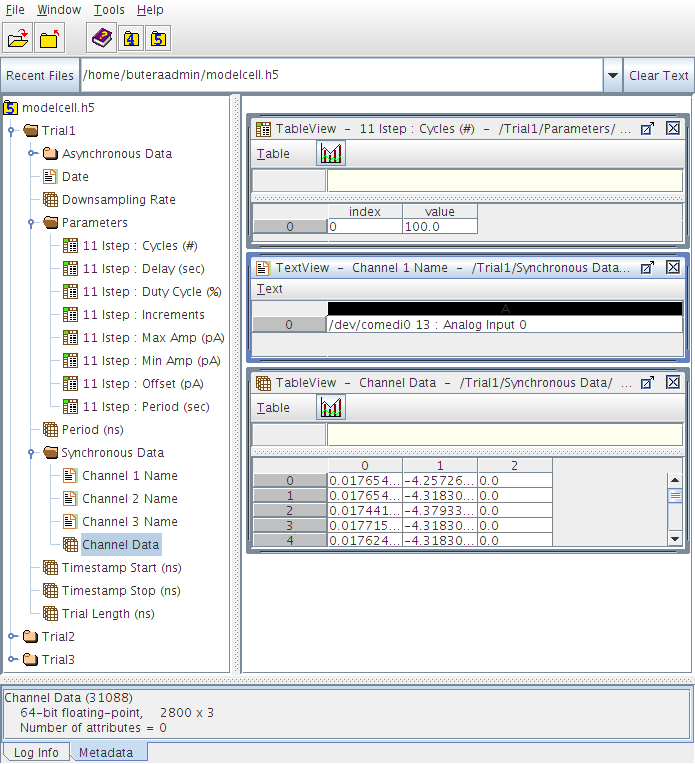
\includegraphics[width=6.5in]{axoclamptutorial5.png} 
\caption[HDF5]{RTXI uses a hierarchical HDF5 data structure organized into \emph{Trials}. Each \emph{Trial} contains the system settings and parameter values for that trial. This screenshot is taken using HDFView, a free software for browsing HDF5 files.} 
\label{fig:HDF5 structure}
\end{center}
\end{maxipage}
\end{figure}

\index{HDF5, MATLAB}There are various software available for working with HDF5 files. To simply browse the file structure, you can use the free HDFView application. HDFView provides some limited editing capabilities. For trials where only a single channel is saved, you can also preview a plot of the data. To extract the data for analysis and for complete editing capabilities, APIs are available for MATLAB, GNU Octave, Igor Pro, Mathematica, Python, Scilab, and other software. \marginlabel{MATLAB \& RTXI HDF5}For real-time streaming of multiple signals, an HDF5 data type is used in RTXI that does not map efficiently onto MATLAB native data types. While MATLAB can read this data using its low-level functions, this process can be very slow. To load RTXI HDF5 files quickly into MATLAB, you will first need to run a small utility function on your HDF5 file to convert the \emph{Synchronous Data} dataset to a different data type. This function is compiled when RTXI is compiled and is located in \texttt{rtxi/hdf}. To convert your HDF5 file:\index{rtxi\_hdf\_matlabize}
\begin{example}
\$ rtxi\_hdf\_matlablize YOUR\_FILE.h5
\end{example}

To make this utility accessible from any directory on your system, make a symbolic link in \texttt{/usr/bin} to the location of this function in your RTXI source directory. If you installed RTXI from the Live CD, the source directory is \texttt{/home/rtxi}:
\begin{example}
\$ sudo ln -s RTXI\_SRC\_DIR/hdf/rtxi\_hdf\_matlabize \\ \hspace{1cm} /usr/bin/rtxi\_hdf\_matlabize
\end{example}

RTXI also includes a simple MATLAB GUI for quickly viewing the data within a single trial. The MATLAB code is available in \texttt{rtxi/hdf/RTXIh5\_MATLAB}. A sample m-file called \texttt{example.m} provides examples of how to extract data to the MATLAB workspace, use the GUI browser, and add new datasets to your file. It is also possible to embed binary formats, such as images, within a trial.

The GUI browser allows you to view the parameters, channels, and plots of the data within a single trial with the \texttt{rtxibrowse()} function. This generates a MATLAB figure window with the filename and trial number in the menu bar. To browse trials within the same HDF5 file, use the buttons in the lower left corner. The left panel lists the initial values for all the module parameters. If a parameter value has changed during the recording, this is denoted with an asterisk. The new values and their timestamps can be viewed by using the \texttt{getTrial()} function, which returns a MATLAB structure containing all the information within a trial. The GUI plots two channels from the same trial. Use the middle upper and and lower panels to select the data that is plotted in the right upper and lower panels. Double-clicking on a channel name in the middle panel will create a new figure window with that data plotted. This allows you to continue browsing through other trials in the main GUI window while keeping this additional plot available.

\begin{figure}[h!]
\begin{maxipage}
\begin{center}
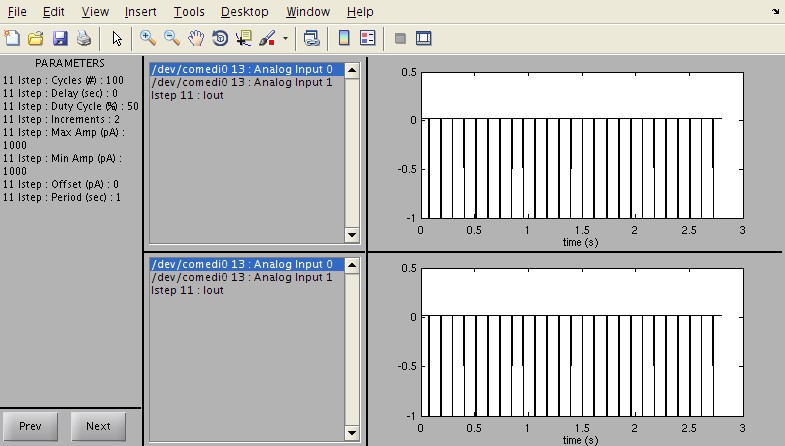
\includegraphics[width=6.5in]{axoclamptutorial6.png} 
\caption[RTXI HDF5 MATLAB GUI]{The MATLAB GUI browser allows you to view the parameters, channels, and plots of the data within a single trial.} 
\label{fig:HDF5 MATLAB}
\end{center}
\end{maxipage}
\end{figure}
